\documentclass[11pt]{article}
\usepackage[utf8]{inputenc}
\usepackage{booktabs}
\usepackage{multicol}
\usepackage{amsmath}
\usepackage{amsfonts}
\usepackage{fullpage}
\usepackage{amsmath,amssymb,amsthm}
\usepackage{tikz,lipsum,lmodern}
\usepackage[most]{tcolorbox}
\usepackage{graphicx}
\def\R{{\mathbb{R}}}
\def\N{{\mathbb{N}}}


\begin{center}
    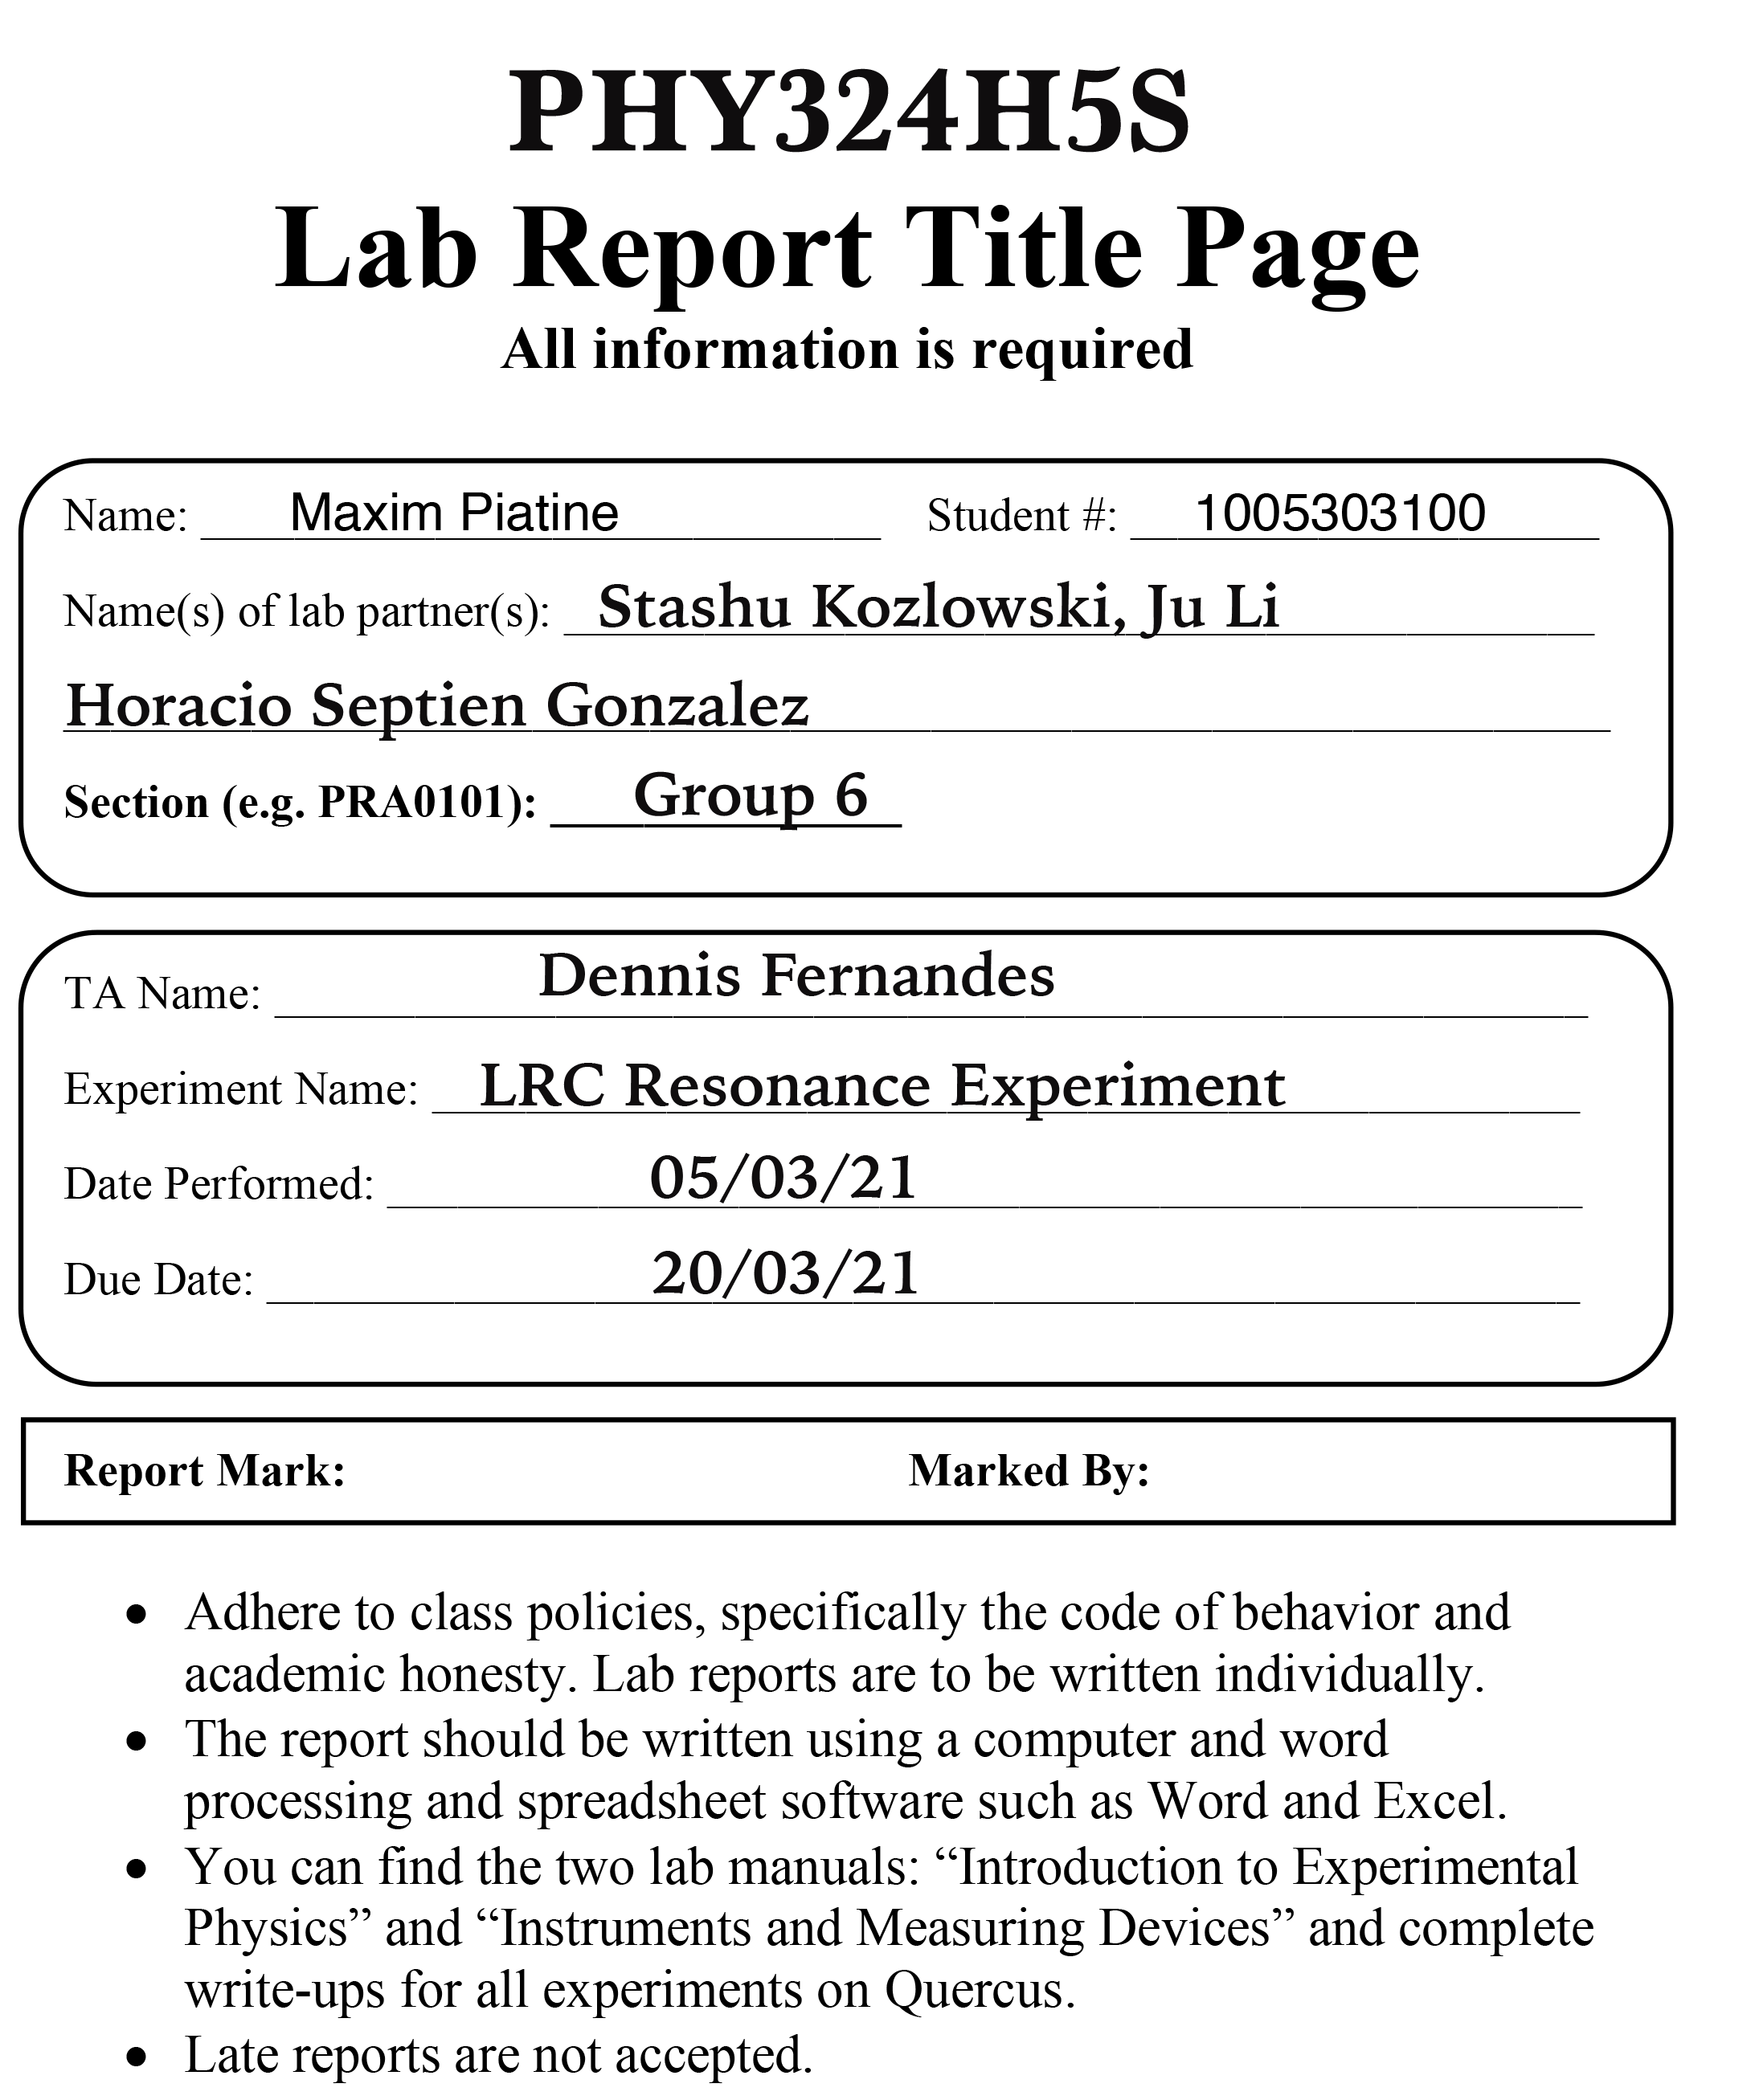
\includegraphics[width=17cm]{cover.png}
\end{center}

\newpage
\begin{document}
\section*{Abstract}
In this laboratory, the purpose was to get familiar with the concepts of resonance, phase shifts of a LRC circuit. Evaluating an LRC circuit depending on the resistance, inductance, and capacitance. As well as, observing the phase difference between applied voltage and the current measured below resonance, at resonance, and above resonance. \\
By evaluating different resonances depending on the resistance, inductance, and capacitance; it is clear that the theoretical formulas are heavily influenced. The resonance frequency is proportional to the inverse of the inductance and the capacitance; thus, depending how large or small the values are, it will fluctuate the resonance frequency based on these values. The larger the capacitance and inductance is the smaller the resonance frequency will be. Also, the smaller the capacitance and inductance are the larger the resonant frequency are. The resistor does not affect the resonant frequency, due to the resistor being equal to the impedance. The resistor affects the maximum current and total voltage. If the resistor is too high then the maximum current will be small, and if the resistor is too small then the maximum current will be bigger in value.\\
The phase difference was calculated using the phase angle between the voltage and current amplitudes. At resonance the current leads the voltage through the capacitor and the voltage carries current through the inductor. Above the resonant frequency, the current leads the voltage and the inductance reactance will be larger than the capacitance reactance. Below resonance the voltage leads the current and the capacitance reactance will be larger than the inductance reactance.\\
From the calculations, the theory and the experimental values followed well with each other. The laboratory was successful. 


\section*{Introduction}
The current through a series LRC circuit is examined as a function of applied frequency and the effects of changing the values of the resistance, inductance, and capacitance are observed. The phase difference between the applied voltage and the current is measured below resonance, at resonance, and above resonance. An inductor, a capacitor, and a resistor are connected in series with a sine wave generator. If the applied voltage is:
\begin{equation}
    J=J_{max}\sin(\omega t)
\end{equation}
then the current in the series LRC circuit is:
\begin{equation}
    I=I_{max}\sin(\omega t + \phi)
\end{equation}
The maximum current and total voltage are then related by:
\begin{equation}
    I_{max}=\frac{E_{max}}{Z}
\end{equation}
Where $Z$ is the impedance and is the AC analog of resistance for the entire circuit. The phase shift is related to the other variables by:
\begin{equation}
    \tan\phi=\frac{X_C-X_L}{R}
\end{equation}
\begin{equation}
    \phi=\frac{\Delta t}{T}\cdot 2\pi 
\end{equation}
Where $\Delta t$ is the time difference between each peak, $T$ is the period of the wave. The impedance $Z$ is given by:
\begin{equation}
    Z=\sqrt{R^2+(X_C-X_L)^2}
\end{equation}
\begin{center}
    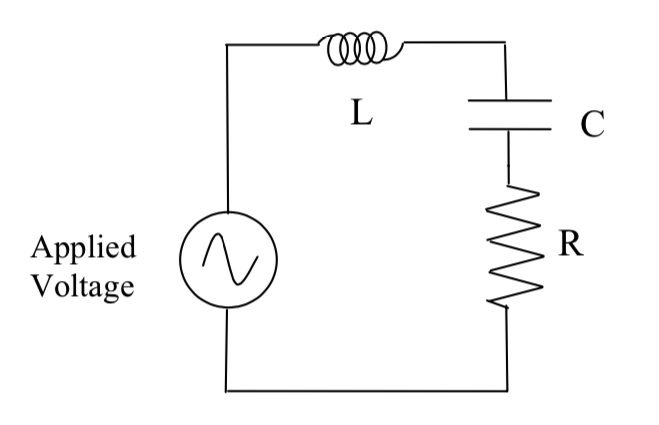
\includegraphics[width=10cm]{1.png}
\end{center}
Since the voltage across the resistor is in phase with the current, the phase of the current can be measured by measuring the phase of the voltage across the resistor.
\begin{equation}
    X_C=\frac{1}{\omega C}=\frac{1}{2\pi fC}
\end{equation}
\begin{equation}
    X_L=\omega L=2\pi fL
\end{equation}
Where $L$ is the inductance measured in henrys $H$, $C$ is the capacitance measured in farads $F$, and $f$ is the frequency measured in hertz $Hz$. At resonance, the current is maximum and thus the impedance is at its minimum. The minimum impedance (6) is equal to $R$ due to $X_L=X_C$. This yields the resonant frequency:
\begin{equation}
    \omega_{res}L=\frac{1}{\omega_{res}C}
\end{equation}
\begin{equation}
    \omega_{res}=\sqrt{\frac{1}{LC}}
\end{equation}

\section*{Procedure}
Follow the "LRC Resonance" Pasco, written by Ann Hanks.\\

\noindent Connect the GLX Power Amplifier to the GLX by plugging the two cables into the side of the GLX. One cable into the GLX on-board voltage sensor port, the other into the external speaker output port. You can identify each cable by the size of the digital plug.\\

\noindent Connect the GLX Power Amplifier to its power supply (the green LED should light).\\

\noindent Open the GLX file called lrc.glx.\\

\noindent Construct the circuit shown below, without the iron core in the coil, the 100 μF capacitor, and the $10\Omega$ resistor in series with the applied voltage.\\

\noindent Turn the GLX Power Amplifier On by navigating to the Output screen on the GLX and pressing F1. You will see that the F1 button is labeled above it as “On.” The relay inside the Power Amplifier should click and the green light inside the case will indicate that the unit has been switched on.\\

\noindent Now navigate back to the Graph screen and press the Start/Stop button on the GLX. The frequency scan will begin. After the current has reached its maximum and has returned to its starting value, press the Start/Stop button on the GLX to stop recording.\\

\noindent Press the Auto Scale (F1) button.

\section*{Data and Analysis}
The purpose of this experiment was to observe the effects of the resistance, inductance, and capacitance. Visualising the resonance frequency of the LRC circuit depending on the resistance, inductance, and capacitance. Also, the phase difference between applied voltage and current below resonance, at resonance, and above resonance.\\
Firstly, the resonance frequency was measured with the help of PASCO capstone. To determine the resonance frequency depending on the resistance, inductance, and capacitance, the experiment replaced all the materials to determine the affect on the resonant frequency. 
\begin{center}
    \textbf{Graph 1}: Resonance of Peak Current against Output Frequency\\
    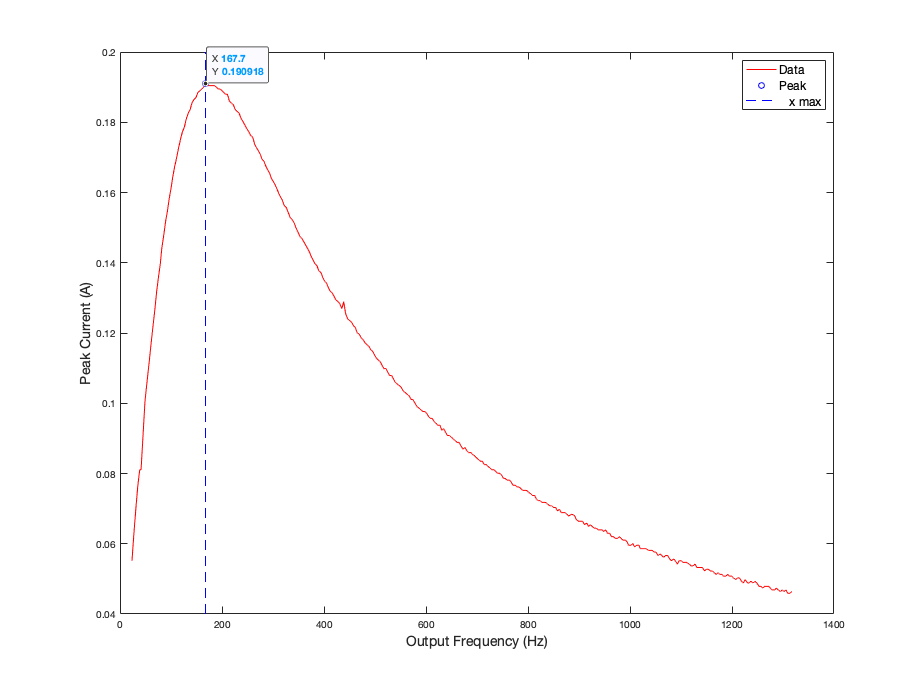
\includegraphics[width=15cm]{Example.png}\\\textbf{Graph 1}: From the raw data collected with $10.2\Omega$ resistor, $97.1\mu F$ capacitance, and $8.2mH$ inductance provided this graph as an example of one of three trials. The independent value $x$ is the output frequency measured in hertz, and the dependent value $y$ is the peak current measured in amperes. The red graph is the collection of data points from this experiment, the blue dot is the peak of the graph sitting at $(167.7,0.190918)$, and the blue dotted line shows the resonance at the peak. The graph presents itself as asymmetric, due to the capacitance and inductive reactance. Since the capacitance reactance formula contains the frequency in the denominator, it makes it easier for the capacitance reactance to decrease as frequency increases. On the other hand, the inductive reactance has frequency in the numerator, as frequency increases the faster inductive reactance increases. 
\end{center}
The resonance frequency will be the peak of the graph from graph 1, the theoretical way of computing the resonance frequency is using the minimum impedance formula with equation (10), where $X_L$ and $X_C$ are equal to each other. Using the known information of the inductance and capacitance of the circuit, it is clear that the resistor does not have an affect on the circuit if it were to be changed. With $10.2 \Omega$ as the resistor, $97.1 \mu F$ as the capacitor, and $8.2mH$ as the inductor inductance; the theoretical value of the resonance frequency would be $178 Hz$. From taking three different trials to determine the experimental value, The experimental value obtained was $178\pm7.45 Hz$ with the help of the average and standard deviation. Giving an error percentage of $0.3\%$. Using the same resistance and capacitance, the inductor inductance is changed to an iron core with $27.1 mH$. The experimental value turned out to be $78.8\pm 0.1 Hz$, and the theoretical value $53.2 Hz$. Giving an error percentage of $20\%$, that being due to the parasitic capacitance between the coils and the iron that affects the frequency resonance. Changing the capacitor to a $330\mu F$ and maintaining the resistor and iron core, knowing that there is still a parasitic capacitance between the coils and the iron core, the experimental value is $40 \pm 1.4 Hz$. Comparing to the theoretical resonance of $53.2 Hz$, the error percentage is at a $25\%$, keeping in mind the reason for such a high error percentage. Now, removing the iron core from the equation and replacing it with the previous inductor the inductance is $8.2 mH$, the capacitance is $330 \mu F$, and resistance the same. The experimental resonance is $100 \pm 3 Hz$, and theoretical is $97 Hz$. The error percentage between theoretical and experimental is $3.6\%$; but, theoretical value lies within the experimental uncertainties. From the collected information, the equation (10) has the inductance and capacitance inversely proportional to each other. The higher the value of capacitance and inductance is, the lower the resonant frequency will be. On the other hand, if the capacitance or the inductance is low, then the resonant frequency will be high. The resistor does not affect the resonant frequency in these calculation.\\

The resistor affects the current amplitude of the circuit, depending how high the resistor is, it may affect the peak of the current. Looking at equation (3), the maximum current is proportional to the impedance; thus, at resonance, the maximum current will be smaller if the resistor is high, and current will be higher if the resistor is smaller. With different resistors attached in parallel, the maximum current will be different. \\

Lastly, the phase difference between the applied voltage and the current is examined for different frequencies. To find the phase shift between the current and the voltage, equation (4) comes in hand. To find the phase angle, with equation (5), the $\Delta t$ can be found via Capstone; the Capstone $\Delta t$ tool can track the time difference between the amplitude peaks between current and voltage. Using the same Capstone tool, can determine the period of current and voltage.
\newpage
\begin{center}
    \textbf{Graph 2}: Resonance of Peak Current against Output Frequency\\
    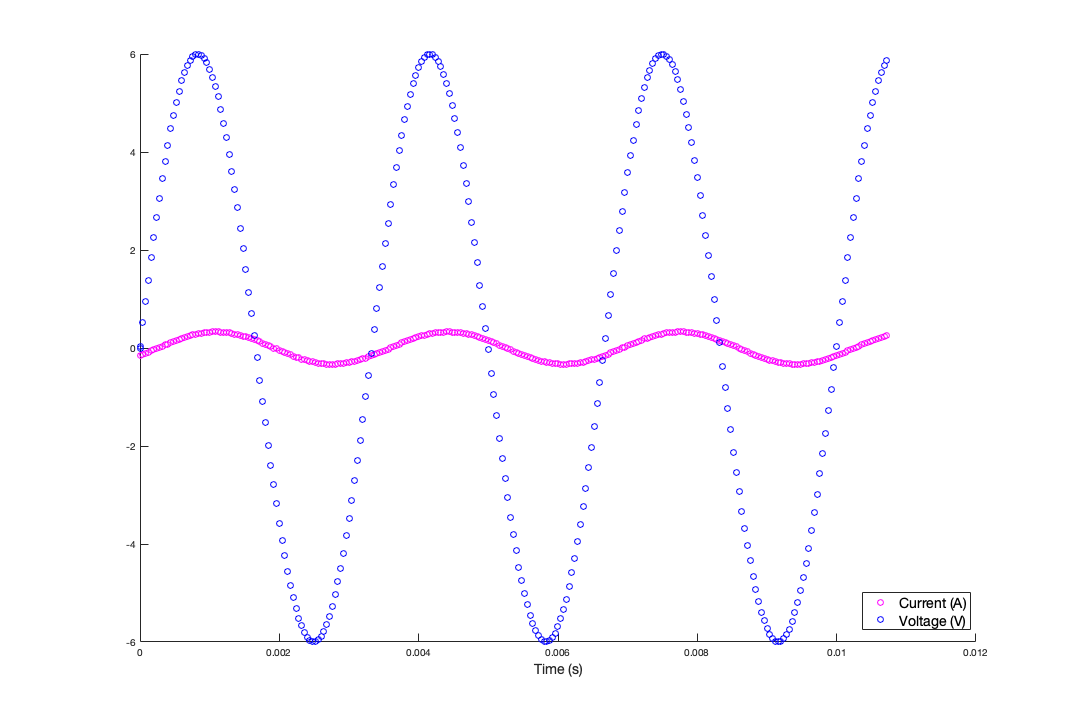
\includegraphics[width=15cm]{G.png}\\\textbf{Graph 2}: From the raw data collected of $300Hz$ frequency. The independent value $x$ is the time measured in seconds, and the dependent value is measured by two graphs; the pink graph is the current measured in amperes represented by a sinusoidal wave between $\pm0.3$ amperes, and the blue graph is the voltage measured in volts represented by a sinusoidal wave from $\pm6$ voltage. 
\end{center}
The experiment consisted of three different frequencies. At $100Hz$, the phase angle obtained between current and voltage was $0.78\pm 0.31$, and the phase shift being $1\pm 0.31$. The theoretical value is calculated to be $1.07$, giving an error percentage of $7\%$ but since the value lies within the uncertainty, makes the experimental value valid. At $300Hz$, the phase shift calculated experimentally between the current and voltage was $-0.94\pm0.005$; which is $7\%$ away from the theoretical value as well being $-1.02$. At resonance, $175Hz$, the phase shift between the current and voltage was $-0.025\pm0.003$, which makes sense considering the space between the current and voltage should be close to zero. The theoretical value was $-0.023$; thus, the value lies within the uncertainty of the experimental. Furthermore, at $175Hz$, the iron core is added to the edition of calculations, the experimental value turns out to be $-1.53\pm0.6$; comparing to the theoretical value of $-2.1$, it lies within the uncertainties. Making these phase shifts completely reasonable. By observing, it seems that the current is leading the voltage in a capacitor and voltage leads current in an inductor. Above the resonant frequency, the inductive reactance gets bigger due to equation (7) getting smaller and equation (8) getting larger. Below resonant frequency, the inductive reactance is smaller and capacitance reactance is bigger. 

\section*{Discussion and Conclusion}
To conclude, e effects of the resistance,  inductance,  and capacitance. Visualising  the resonance frequency of the LRC circuit depending on the resistance,inductance, and capacitance. Also, the phase difference between applied voltage and current below resonance, at resonance, and above resonance.\\
The resonance depending on the resistance, only affects the impedance. The impedance would only equal the resistor value, depending on how high the resistor value would be, the lower the peak current would be, since the maximum peak is proportional to the resistance (equation (3)). When looking at the capacitance and the inductance, following the equation (10), no matter what value is in place for the inductance and capacitance, the resonant frequency will fluctuate depending on these value. If the values of inductance and capacitance are really small then the resonant frequency will be very large. If the capacitance and inductance are very large then the resonant frequency will be very small. That being said, using different values of capacitance and inductor cores. From the values obtained, the $20\%$ and $25\%$ errors are due to the parasitic capacitance between the coils and the iron core. Every other value obtained without the iron core; the theoretical values were inside the experimental ones. \\
The phase difference between the applied voltage and current was examined with different frequencies. Depending the frequency, it affected the phase shift. If the value was smaller than the resonant frequency then the phase shift would be from the voltage leading the current. If the value was larger than the resonant frequency then the phase shift would be negative due to the current leading the voltage. At resonance the current was leading the voltage in a capacitor and voltage leads current in an inductor. Below resonance, the inductive reactance is smaller and capacitance reactance is bigger. Moreover, below resonance the voltage leads the current. Above resonance, the capacitance reactance is smaller than the inductive reactance. Furthermore, above resonance the current leads the voltage. 
\newpage
\section*{Appendix}
Wagih, Ghobriel: Lab manual I: Introduction to Experimental Physics.
Ann Hanks,"LRC Resonance" Pasco.

\begin{center}
\caption{\textbf{Table 1}: Table of Information Output Frequency, Peak Current, and Averages} 
 \begin{tabular}{||c c c c c||} 
 \hline
 Runs & Peak Current (A) & Output Frequency (Hz) & Average & Standard Deviation\\ [0.5ex] 
 \hline\hline
 Run 17 & 0.19 & 167.7 & 177.975 (Hz) & 7.454025758 (Hz) \\ 
 \hline
 Run 18 & 0.19 & [177.8, 181.4] & & \\
 \hline
 Run 19 & 0.19 & 185 & & \\ [1ex] 
 \hline
\end{tabular}
\\\textbf{Table 1}: From the collected results of peaks and output frequencies, the average and standard deviation was calculated. $10.2 \Omega$ as the resistor, $97.1 \mu F$ as the capacitor, and $8.2mH$ as the inductor inductance, will be used to calculate the experimental resonance.
\end{center}
Calculations of Output Frequencies:
\[\bar X= \frac{1}{N}\sum^N_{i\in\N}X_i=\frac{167.7+177.8+181.4+185}{4}=177.975\]
Standard deviation uncertainty of average:
\[s=\sqrt{\frac{\sum^N_{i\in\N}(X_i-\bar X)^2}{N-1}}=\sqrt{\frac{1}{3}((167.7-177.975)^2+...+(185-177.975)^2)}\]\[s=7.454025758\]
The experimental resonance $178\pm7.45 Hz$.
The theoretical Resonance with $10.2 \Omega$ as the resistor, $97.1 \mu F$ as the capacitor, and $8.2mH$ as the inductor inductance:
\[\omega_{res}=\frac{1}{\sqrt{LC}} \Rightarrow f=\frac{1}{2\pi \sqrt{LC}}=\frac{1}{2\pi \sqrt{0.0000971\cdot 0.0082}}=178.454432 Hz\]
The theoretical resonance is $178 Hz$.
Error percentage between theoretical and experimental:
\[\frac{|theoretical-experimental|}{experimental}\cdot 100\% =\frac{|177.975-178.454432|}{178.454432}\cdot 100\%=0.268657936\%\]
The other calculations regarding changing the capacitance, resistance, and inductance are the same process of calculations, just different value.
\newpage
\begin{center}
\caption{\textbf{Table 2}: Table of Information on Different Capacitance and Inductors} 
 \begin{tabular}{||c c c c c||} 
 \hline
 Runs & Exp Resonance (Hz) & Theo Resonance (Hz) & Error Percentage &\\ [0.5ex] 
 \hline\hline
 With iron core at $100 \mu F$ & $78.8\pm0.1$ & 98.11 & $19.6843\%$ & \\ 
 \hline
 With iron core at $330 \mu F$ & $39.98\pm1.4481$ & 53.22 & $24.8784\%$ & \\
 \hline
 Without iron core at $330 \mu F$ & $100.28\pm2.5459$ & 96.75 & $3.6473\%$ & \\ [1ex] 
 \hline
\end{tabular}
\\\textbf{Table 2}: From the collected results of peaks and output frequencies, the collected. For different runs of inductors and capacitance, the different results of experimental and theoretical values. As well as, their respective their error percentage.
\end{center}
\begin{center}
\caption{\textbf{Table 3}: Table of Information with Phase Shifts} 
 \small\begin{tabular}{||c c c c c||} 
 \hline
 Runs & $\Delta t$ & Period $T$ & Average $\Delta t$ &\\ [0.5ex] 
 \hline\hline
 $100 Hz$ freq & [0.00098, 0.00099, 0.00098] & [0.01, 0.01, 0.005] & $9.833\cdot10^{-4}\pm 5.7 \cdot 10^{-6}$  &\\ 
 \hline
 $300 Hz$ freq  & [-0.0004, -0.0004, -0.0004] & [0.0034, 0.0033, 0.0033] & -0.0004  & \\
 \hline
 $178 Hz$ freq  & [$-2.5\cdot10^{-5}$, $-2.1\cdot10^{-5}$, $-2.1\cdot10^{-5}$] & [0.00555,0.00569, 0.00563] & $-2.23\cdot10^{-5}\pm 2.31\cdot10^{-6}$  &\\ [1ex] 
 \hline
\end{tabular}
 \small\begin{tabular}{||c c c c c c||} 
 \hline
 Average $T$ & $\frac{\Delta t}{T}\cdot 2\pi$  & Theo Value & $tan\phi$ & Error $\%$ &\\ [0.5ex] 
 \hline\hline
 $7.51\cdot 10^{-3}\pm 2.89\cdot10^{-3}$ & $0.786\pm 0.31$ & 1.076 & $1 \pm 0.316$ &. $6.89\%$&\\ 
 \hline
 $0.00333\pm 2.3\cdot10^{-5}$ & $-0.75\pm0.005$ & -1.015 & $-0.94\pm0.005$ & $7.5\%$ &\\
 \hline
 $0.0056\pm 4\cdot10^{-5}$ & $-0.025\pm0.003$ & -0.023 & $-0.025\pm 0.003$ & $9.14\%$ &\\ [1ex] 
 \hline
\end{tabular}
\\\textbf{Table 3}: From the collected results, the computed values and theoretical values are presented.
\end{center}
Uncertainty of between $\Delta t$ and $T$:
\[|\Delta t|\sqrt{(\frac{\Delta t}{\Delta t})^2+(\frac{\Delta T}{T})^2}\]


\end{document}